\section{\K 功率因数及其提高}
\Par 一方面,在电能的传递中,由于用电器里存在储能元件,部分的视在功率转换成了无功功率,一部分能量时而从发电厂传到用电端,时而从用电端传到发电厂,对能量的利用率不够;另一方面,无功功率会增加到线上的电流,让能量在导线上的损耗增加.因此,减少无功功率势在必行.

\Par 根据式\ref{equ:功率因数},我们定义了\textbf{功率因数}
\begin{equation}
    \cos \varphi =\frac{P}{S}
\end{equation}
由于我们的视在功率(相当于用电器的功率)不能降低,因此让无功功率减少,就相当于增加有功功率,也就相当于提高功率因数.那么在视在功率$S$一定的情况下,我们如何提高功率因数呢?其实,就是我们要降低$\varphi $值,让电路尽量的往阻性电路靠拢.

\begin{wrapfigure}{r}{0.25\textwidth}
    \centering
    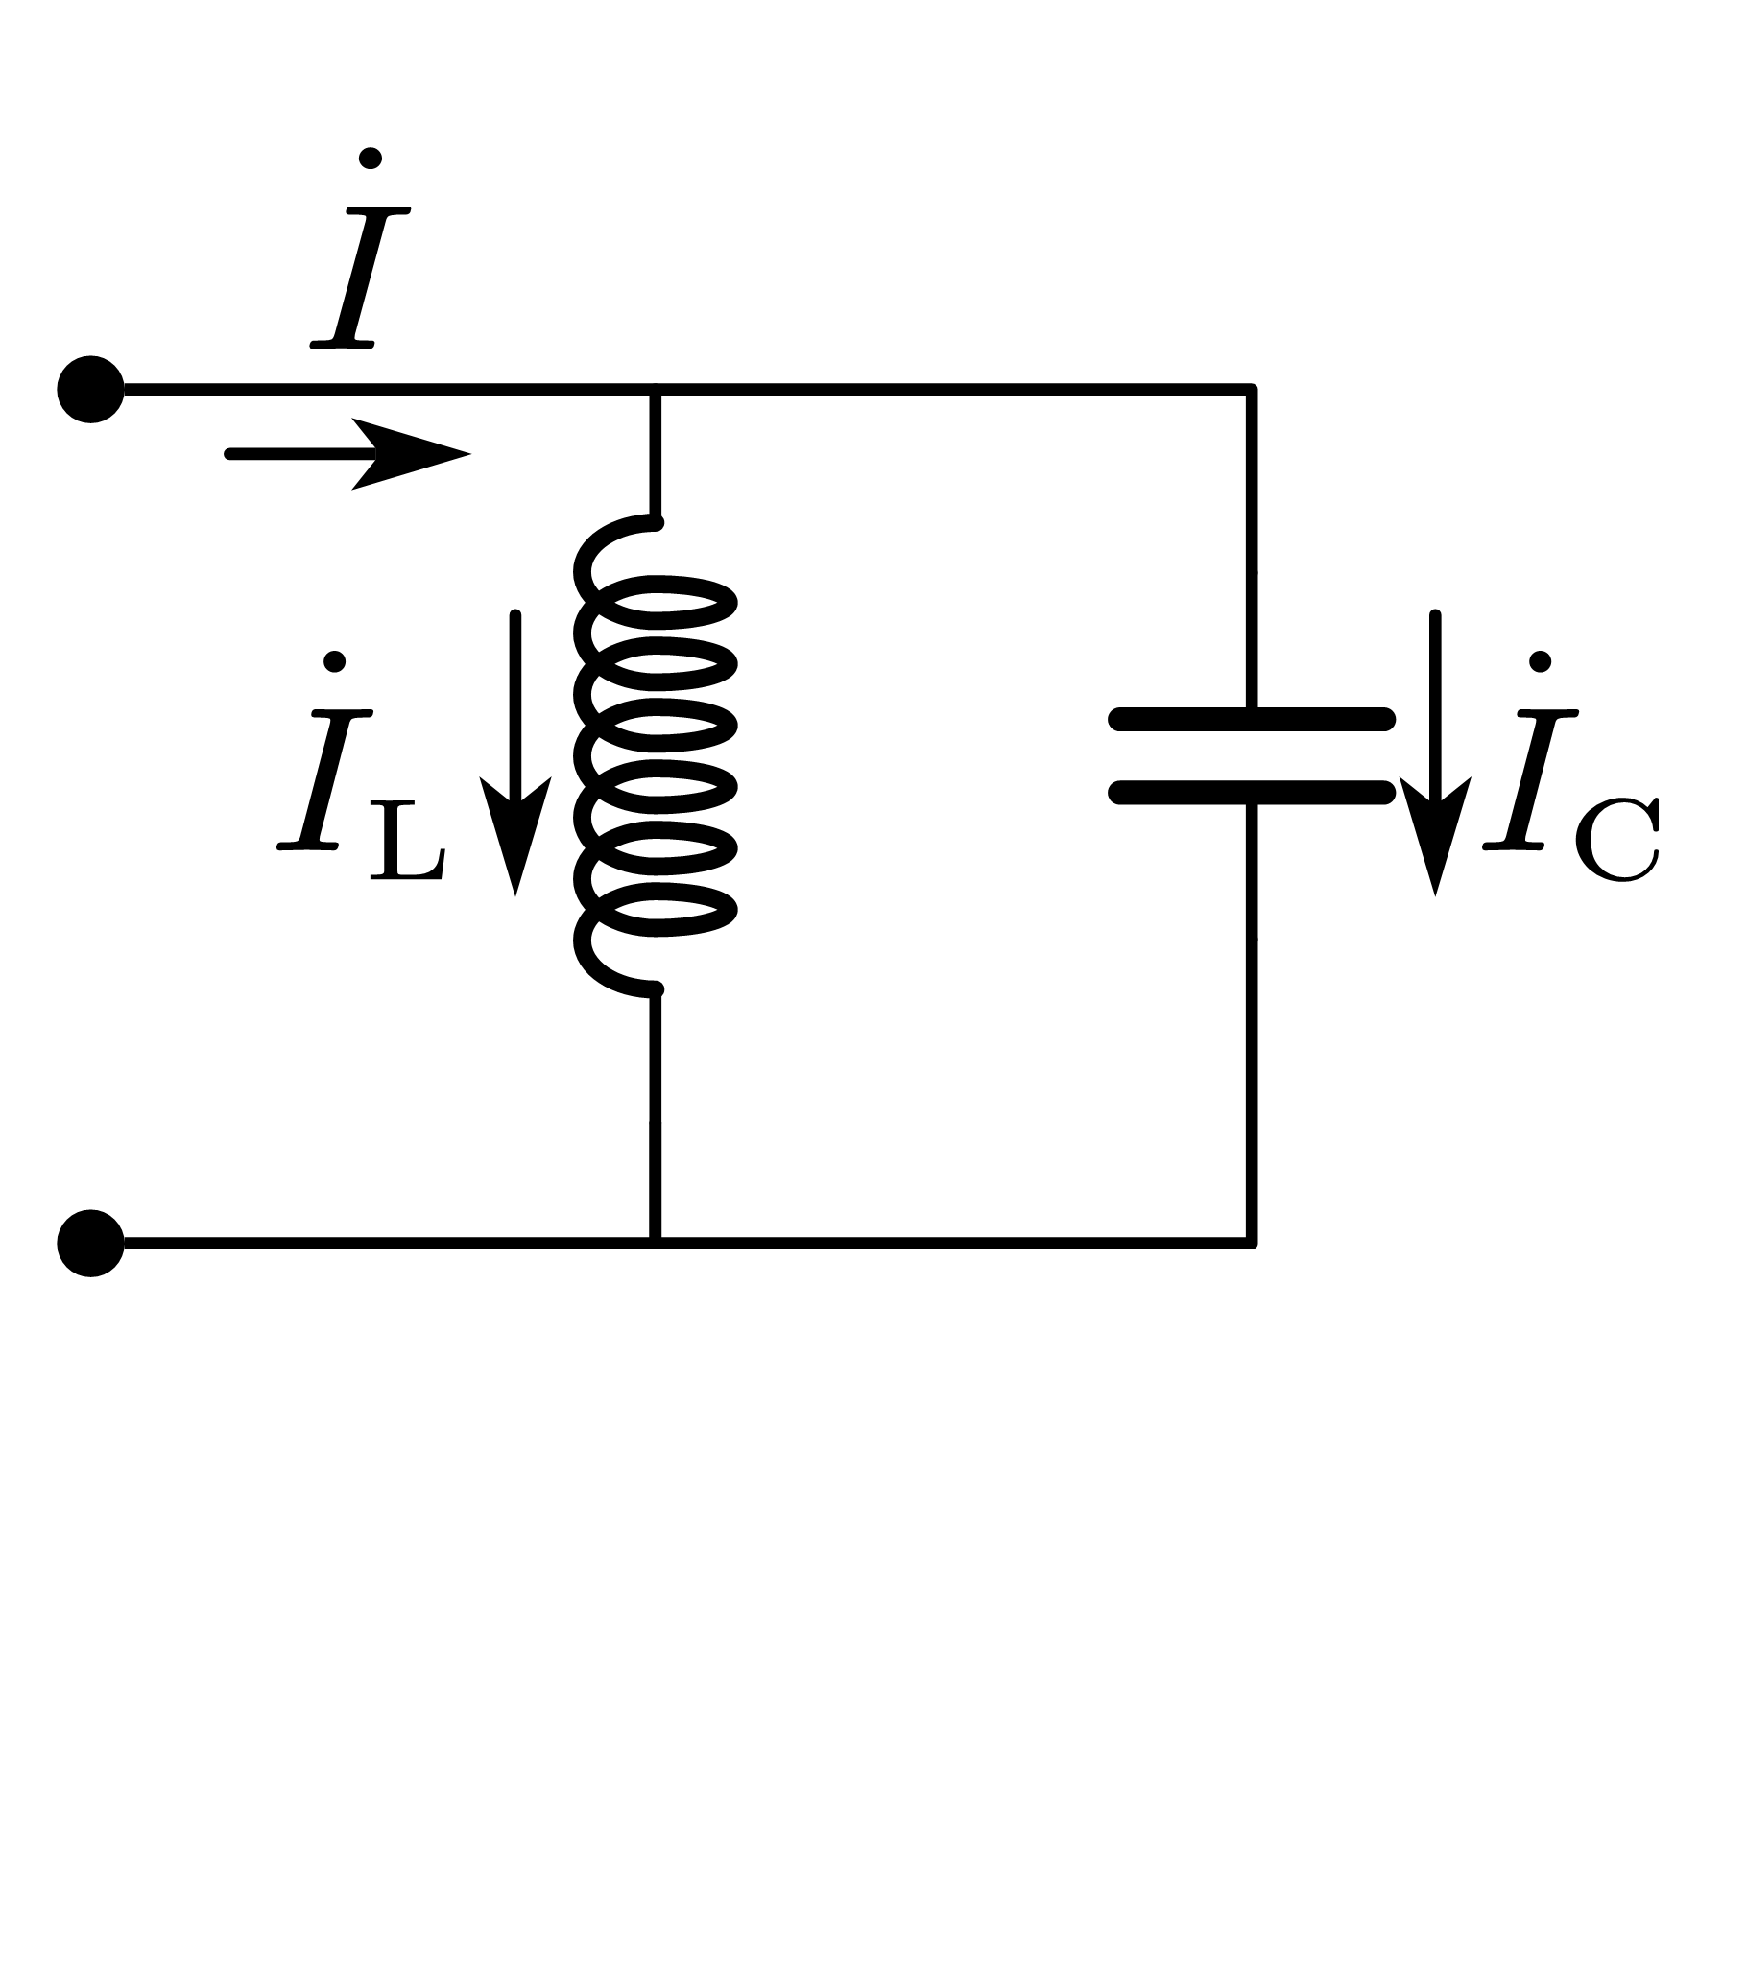
\includegraphics[width=0.25\textwidth]{功率因数电路.pdf}
    \caption{功率因数}
    \label{fig:功率因数电路}
\end{wrapfigure}
\Par 事实上,我们一般用电器里面储能元件大多为电感,因此,为了让电路尽量的往阻性电路靠拢,我们需要往电路里面添加容性元件,那么现在就有两种选择:串联一个适当的电容或并联一个适当的电容.

\Par 经过分析,我们不难知道,串联一个电容是不恰当的,因为串联的电容将会分走电感用电器上的电压,这改变了用电器的功率,违背了我们的初心.因此,我们要选择并联一个电容.

\Par 如图\ref{fig:功率因数电路}所示,我们知道干路电流与支路电流之间的关系为
\begin{equation*}
    \dot{I}=\dot{I}_{\mathrm{L}}+\dot{I}_{\mathrm{C}}
\end{equation*}
我们可以用平行四边形法则进行计算
\begin{figure}[htbp]
	\centering
	\begin{minipage}{0.18\textwidth}
        \centering
        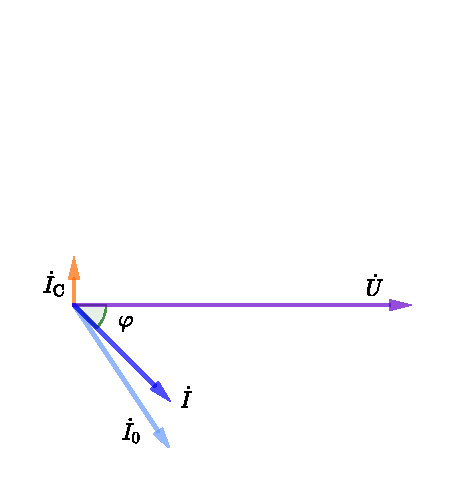
\includegraphics[width=0.95\textwidth]{功率因数的提高1.pdf}
        $C=1\mathrm{\mu F}$
    \end{minipage}
    \begin{minipage}{0.18\textwidth}
        \centering
        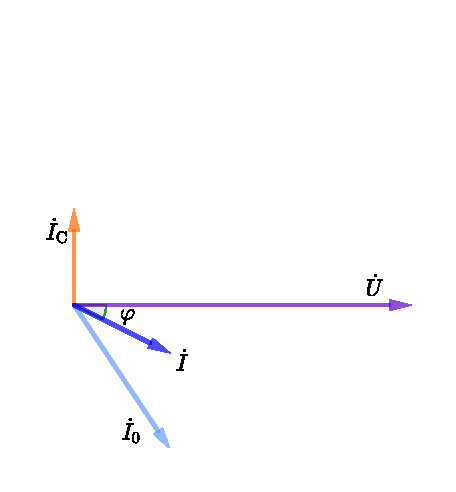
\includegraphics[width=0.95\textwidth]{功率因数的提高2.pdf}
        $C=3\mathrm{\mu F}$
    \end{minipage}
    \begin{minipage}{0.18\textwidth}
        \centering
        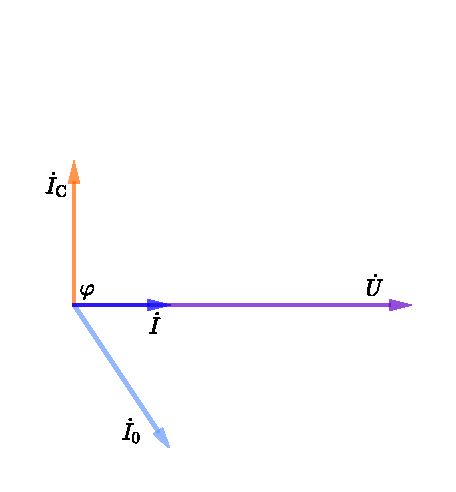
\includegraphics[width=0.95\textwidth]{功率因数的提高3.pdf}
        $C=5\mathrm{\mu F}$
    \end{minipage}
    \begin{minipage}{0.18\textwidth}
        \centering
        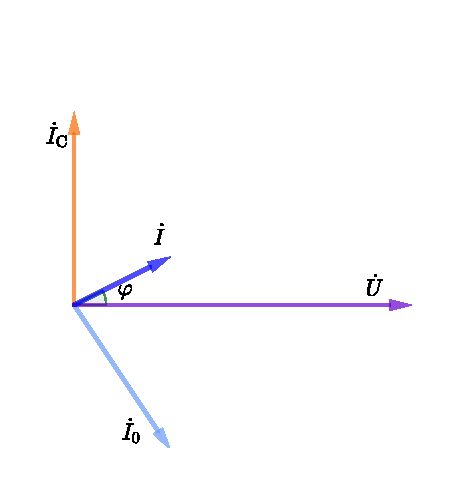
\includegraphics[width=0.95\textwidth]{功率因数的提高4.pdf}
        $C=7\mathrm{\mu F}$
    \end{minipage}
    \begin{minipage}{0.18\textwidth}
        \centering
        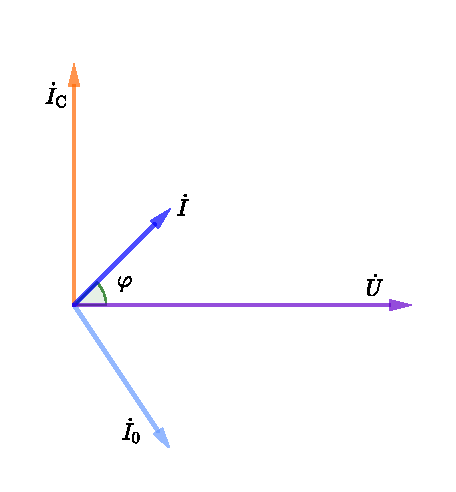
\includegraphics[width=0.95\textwidth]{功率因数的提高5.pdf}
        $C=9\mathrm{\mu F}$
    \end{minipage}
\end{figure}

可以发现,随着补偿电容的增大,功率因数$\cos \varphi $先增大、后减小,因此我们要选择恰当的补偿电容,防止出现过补偿的现象.那么如何计算所需要的补偿电容呢?

\begin{figure}[htbp]
	\centering
	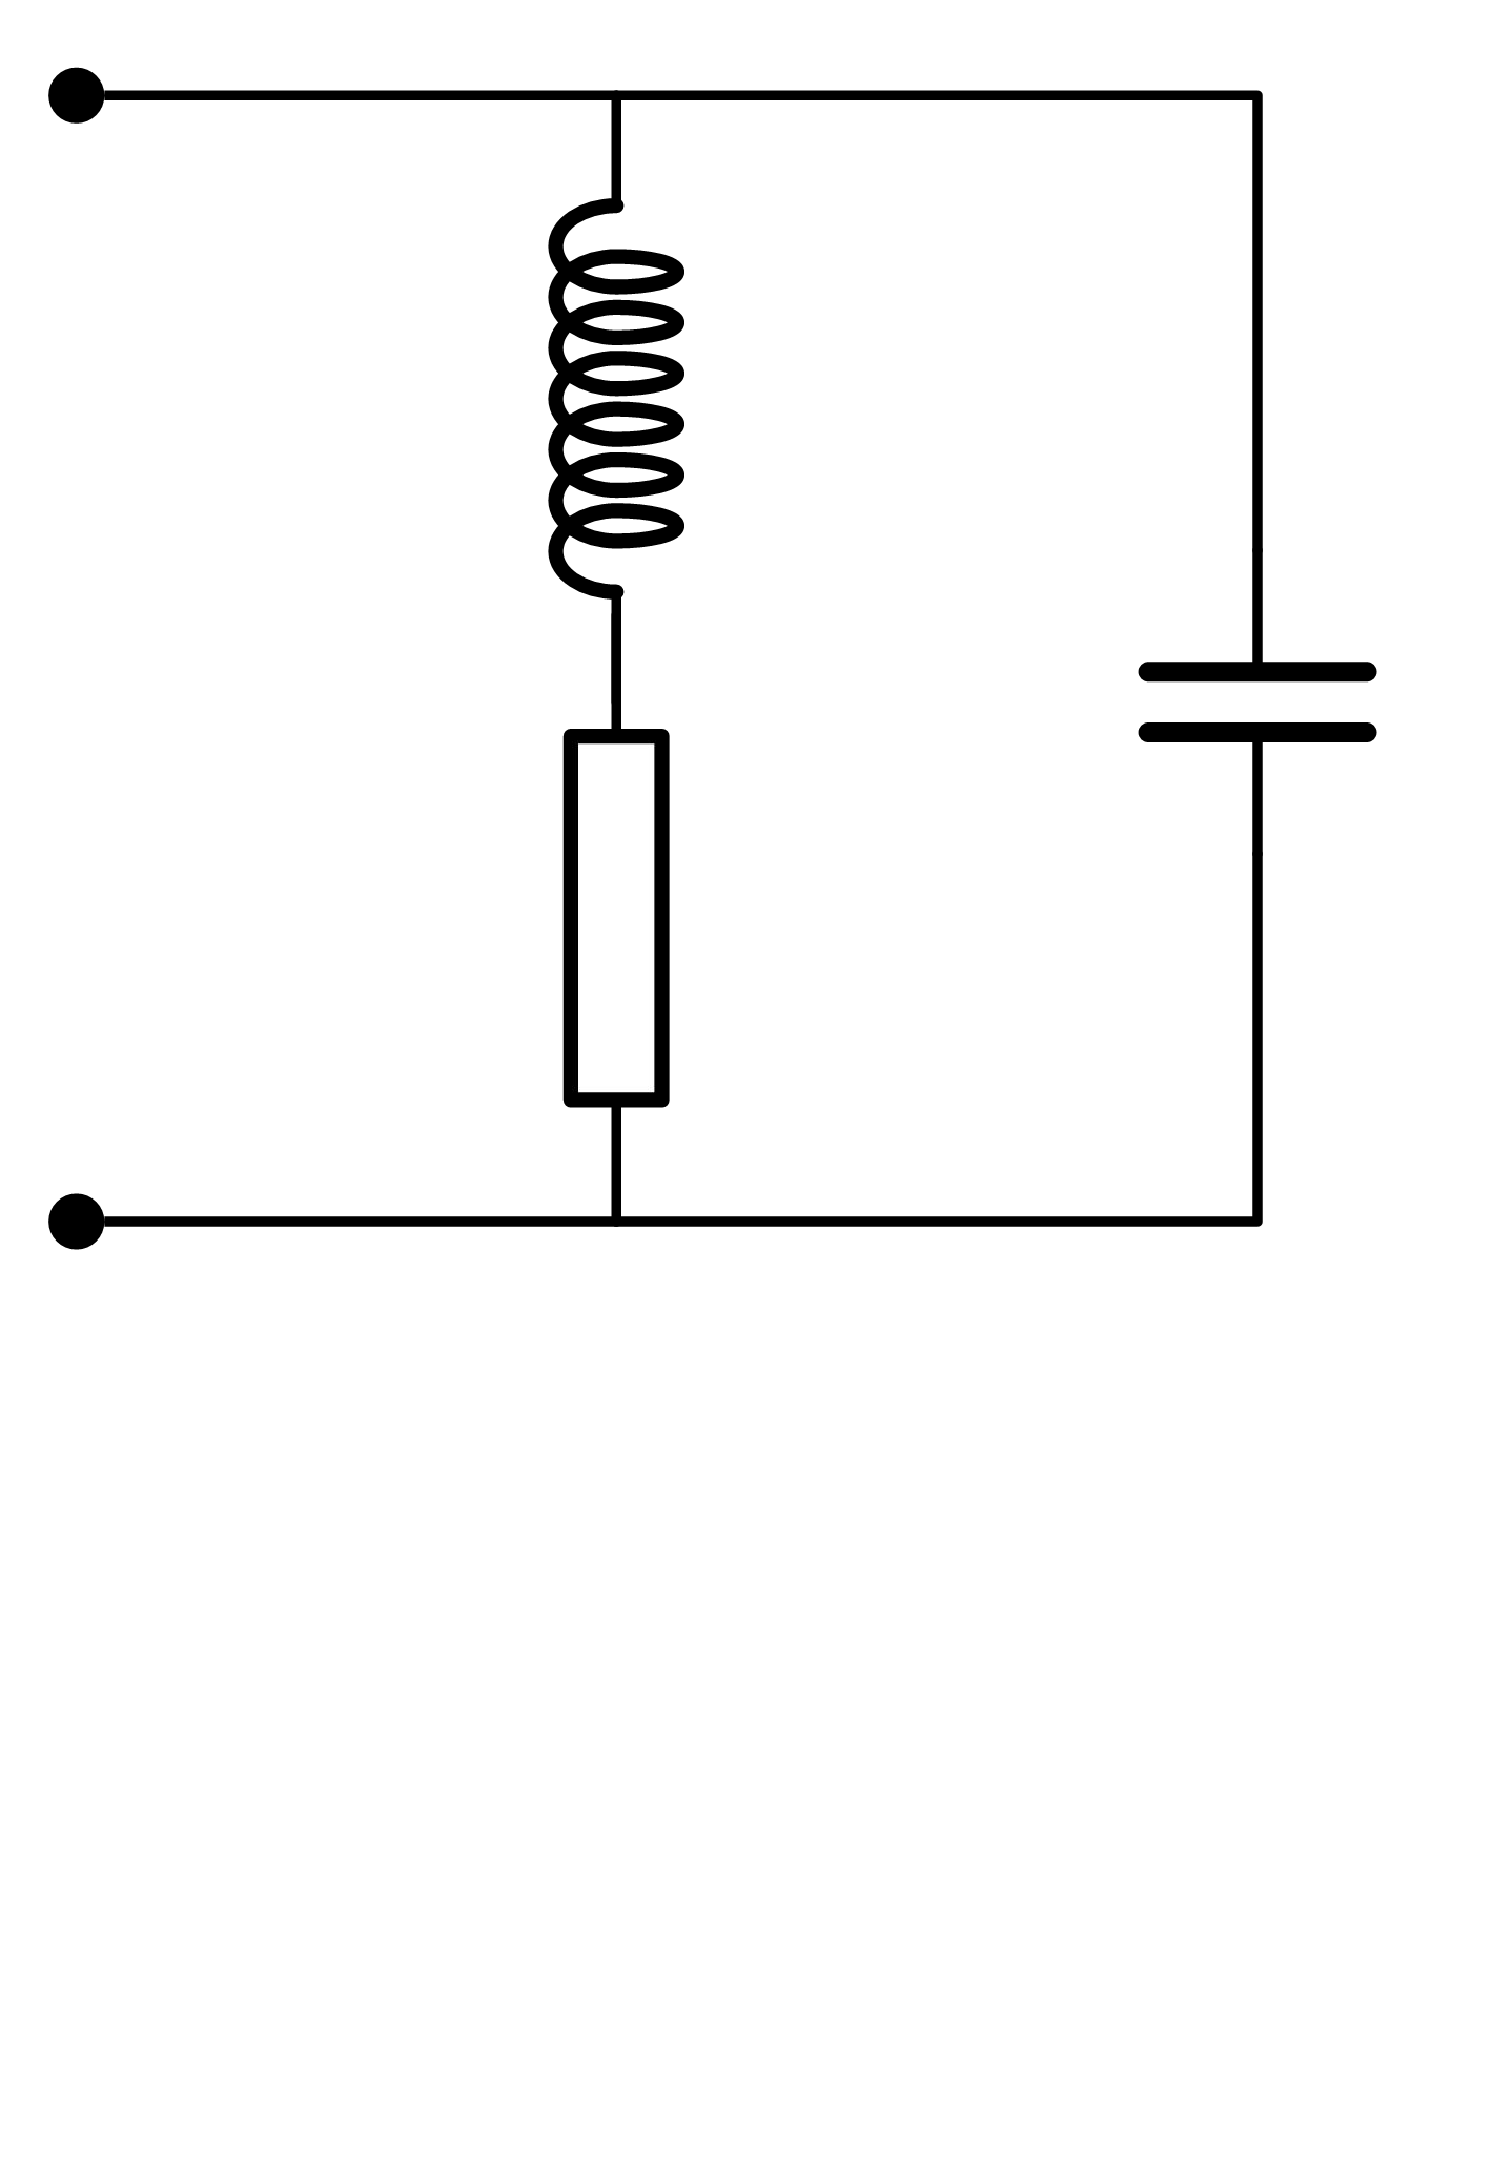
\includegraphics[width=0.25\textwidth]{补偿电容电路}
	\caption{}
	\label{fig:补偿电容电路}
\end{figure}

\Par 设电路如图\ref{fig:补偿电容电路}所示,我们已知电源电压$U$,电源频率$\omega $和有功功率$P$,根据
\begin{equation*}
    \dot{I}=\dot{I}_{\mathrm{L}}+\dot{I}_{\mathrm{C}}
\end{equation*}
可以知道
\begin{equation*}
    I_C=I\sin \varphi -I'\sin \varphi '
\end{equation*}
其中,$I$表示补偿前干路电流,$I'$表示补偿后干路电流.同时我们有
\begin{equation*}
    I=\frac{P}{U\cos \varphi},I'=\frac{P}{U\cos \varphi '}
\end{equation*}
而电容支路电流等于
\begin{equation*}
    I_C=\frac{U}{X_{\mathrm{C}}}=U\omega C
\end{equation*}
结合上式可以得到
\begin{equation}
    C=\frac{1}{U\omega}\left( \frac{P}{U\cos \varphi}\sin \varphi -\frac{P}{U\cos \varphi '}\sin \varphi ' \right) =\frac{P}{\omega U^2}\left( \tan \varphi -\tan \varphi ' \right) 
\end{equation}




